\documentclass[a4paper, 10pt, twoside]{report}


\usepackage[english, dutch]{babel}		% both English and Dutch can be used

\usepackage[a4paper]{geometry}  % margins
\usepackage{setspace}  % spacing between lines
\usepackage{fancyhdr}  % pagestyle
\usepackage[parfill]{parskip}  % set \indent to \\ \\

%% Chapters (layout)
\usepackage{pdfpages}  % include PDF (frontpage)
% \usepackage{natbib}  % style of references
\usepackage[hidelinks]{hyperref}
\usepackage{datatool}
\usepackage{glossaries}
\usepackage[titletoc]{appendix}
\usepackage{titlesec}

%% Tables
\usepackage{tabularx}
\usepackage{longtable}
\usepackage{ltxtable}
\usepackage{booktabs}
\usepackage{multirow}

\usepackage{amsmath}
\usepackage{eurosym}
\usepackage{courier}  % listings font
\usepackage{listings}

\usepackage{rotating}
\usepackage{subfigure}
\usepackage{comment}
\usepackage{pbox}
\usepackage{calc}


% == Landscape =================================================================
\usepackage{pdflscape}  % turn the page also in the PDF
% \usepackage{lscape}  % do not turn the page in the PDF
% ==============================================================================

\usepackage{color}  % listings colors

\definecolor{gray95}{gray}{0.95}
\definecolor{gray50}{gray}{0.5}



\newcommand{\titleinfo}{$ < $ Title $ > $}
\newcommand{\authorinfo}{$ < $ Author $ > $}

\pagestyle{fancy}
\cfoot{}
\fancyhead[RE]{\small\bf\nouppercase\rightmark}
\fancyhead[LO]{\small\bf\nouppercase\leftmark}
\fancyhead[LE, RO]{\thepage}
\renewcommand{\headrulewidth}{0pt}
\setlength{\headheight}{15pt}

\titleformat{\chapter}{\Huge\bfseries}{\thechapter.}{20pt}{}
\titlespacing*{\chapter}{0pt}{15pt}{10pt}

% \setlength{\parskip}{2mm}
% \onehalfspacing

\renewcommand{\maketitle}
{
	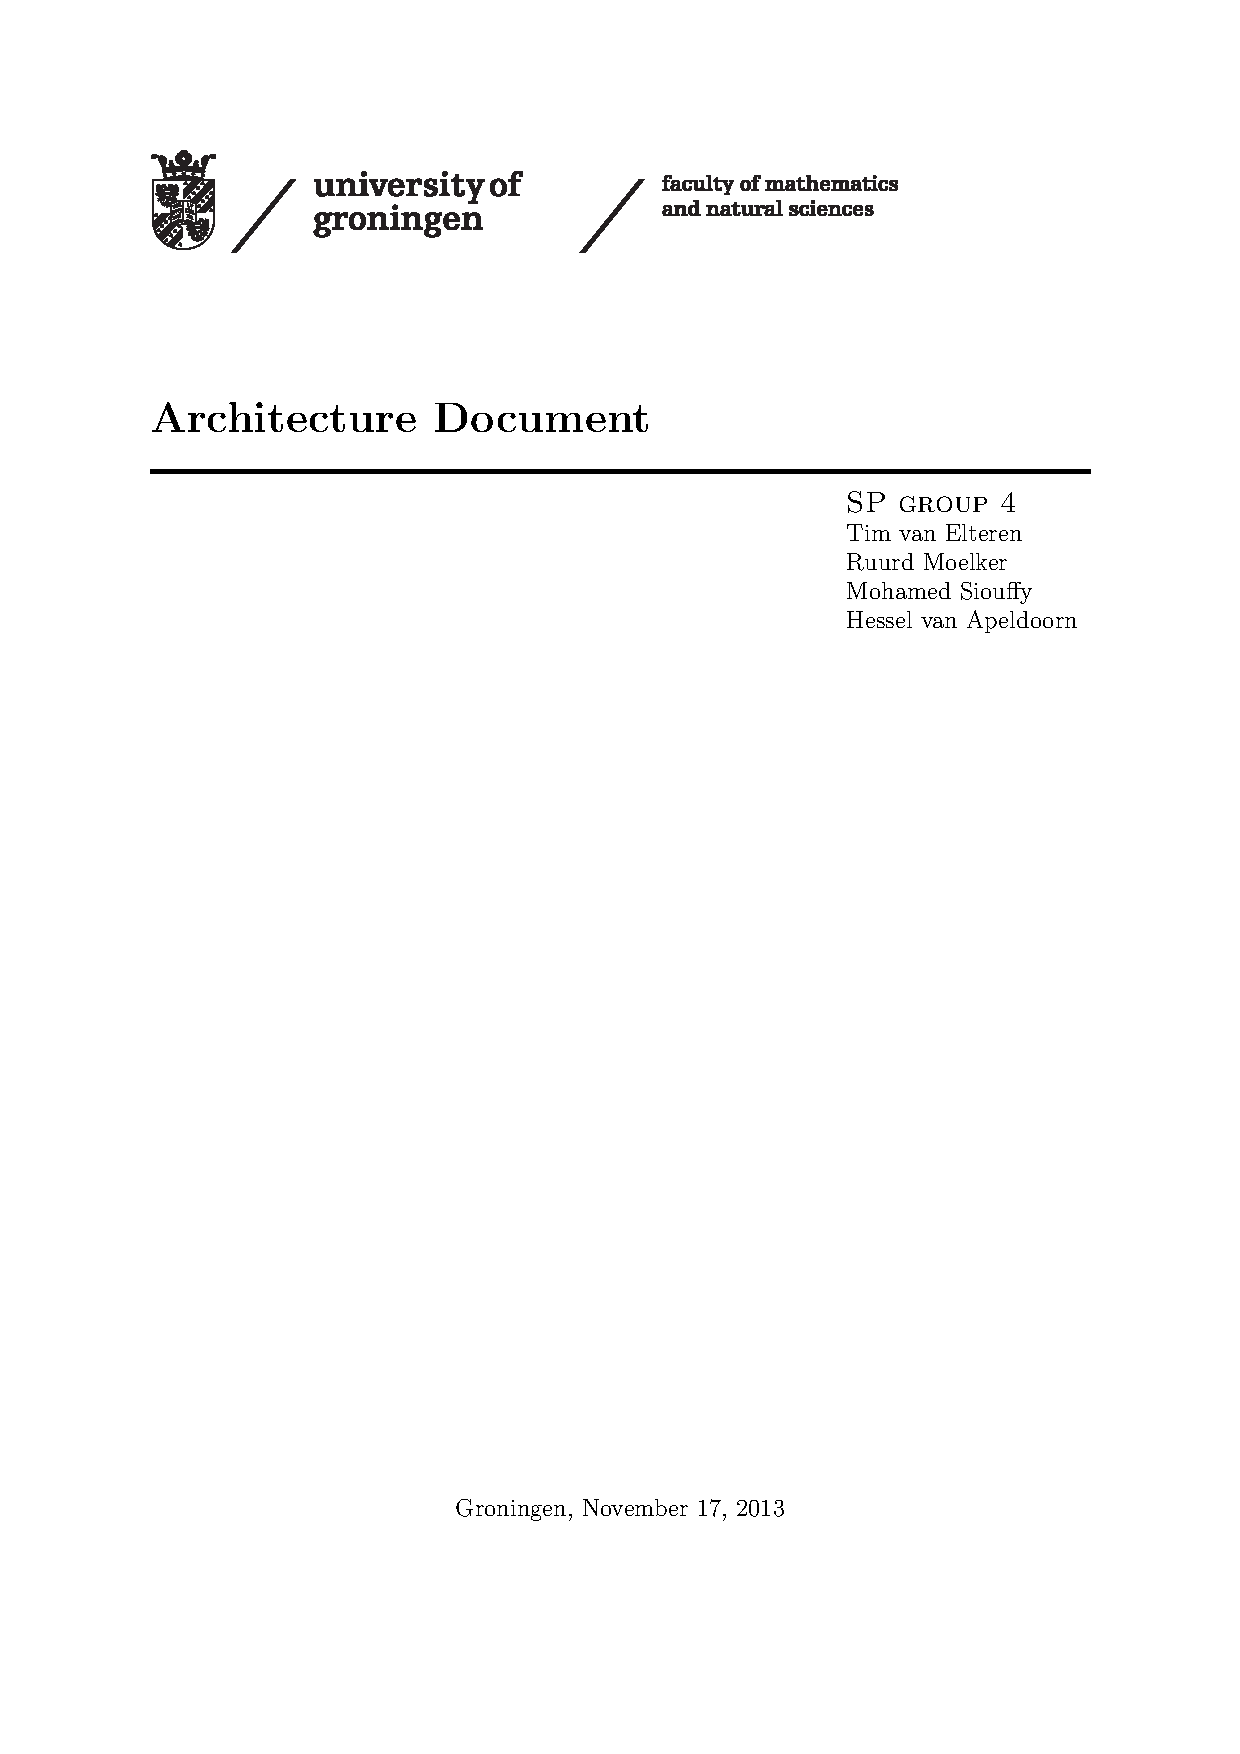
\includepdf{frontpage/frontpage.pdf}
	\thispagestyle{empty}
	% \cleardoublepage
	\pagenumbering{roman}
}

\newcommand{\mytableofcontents}
{
	\renewcommand{\contentsname}{Table of Contents}
	% \addcontentsline{toc}{chapter}{\contentsname}
	\tableofcontents
}

\newcommand{\mylistoffigures}
{
	\listoffigures
	\addcontentsline{toc}{chapter}{List of Figures}
}

\newcommand{\myglossaries}
{
	\glstoctrue
	\printglossaries
	% \addcontentsline{toc}{chapter}{Glossary}
}

\newcommand{\mylistoftables}
{
	\listoftables
	\addcontentsline{toc}{chapter}{List of Tables}
}

\lstset
{
	basicstyle = \fontsize{7pt}{7}\ttfamily,
	keywordstyle = \color{black}\bfseries,
	backgroundcolor = \color{gray95},
	commentstyle = \color{gray50},
	numbers = left,
	language = C++,
	frame = top + left,
	numberstyle = \tiny,
	breaklines = true,
	showspaces = false,
	showstringspaces = false,
	showtabs = false,
	tabsize = 2,
	caption = \tt\lstname,
	xleftmargin = 0pt,
	framexleftmargin = 4pt,
	numbersep = 14pt,
}

\newcommand{\illst}{\lstinline[basicstyle = \ttfamily]}  % prevent small size of inline listing

\glossarystyle{altlist}

\renewcommand{\labelitemi}{$ \circ $}  % ◦
\renewcommand{\labelitemii}{$ \cdot $}  % ·


\renewcommand{\titleinfo} {Active Life for Old Adults}
\renewcommand{\authorinfo}
{
	Tim van Elteren \\
	Ruurd Moelker \\
	Mohamed Elsiouffy \\
	Hessel van Apeldoorn
}

\title{\titleinfo}
\author{\authorinfo}

\makeglossaries

\begin{document}

\makeatletter
\renewcommand*\l@figure{\@dottedtocline{1}{1.5em}{4.5em}}% 3em instead of 2.3em
\let\l@table\l@figure
\makeatother

\selectlanguage{english}			% use English

\maketitle


\chapter*{Authors}
%
\begin{tabularx}{\textwidth}{lXr}%{@{}p{.25\textwidth} p{.45\textwidth} X}
\toprule
\bf Name 					& \bf e-mail & \bf s-number \\
\toprule
	Tim van Elteren 		& {\tt timvanelteren@gmail.com} 			& 1849948\\
	Ruurd Moelker 	& {\tt r.r.moelker@student.rug.nl} 			& 1720678\\
	Mohamed Elsiouffy 	& {\tt m.el.Sioufy@student.rug.nl} 			& 2582678\\
	Hessel van Apeldoorn & {\tt h.b.van.apeldoorn@student.rug.nl} 					& 1881140\\
\bottomrule
\end{tabularx}

zzzzzzz

\begingroup
\let\cleardoublepage\relax
\let\clearpage\relax

\chapter*{Revision History}
\endgroup

\LTXtable{\textwidth}{tables/ltxrevhist.tex}
{\vspace{-.5cm}
\footnotesize Legend: \\
version = yyyy.mm.dd \\
r = reviewed}


\mylistoffigures
\mylistoftables

\mytableofcontents


\newglossaryentry{AAL}
{
	name = {AAL systems},
	description = {Ambient Assistent Living systems are systems designed to to improve the quality of life of the elderly and to reduce the cost of healthcare}
}


\chapter*{Introduction}
\addcontentsline{toc}{chapter}{Introduction}
\pagenumbering{arabic}
For the first assignment of the Software Patterns course we have chosen the subject ``Bookflix''. This document shows the software architecture of this subject. 


The Bookflix idea is loosely based on the streaming service Netflix. Rather than offering video streams, Bookflix offers books. From the Bookflix website, customers can pick a book that they like. This book is then downloaded to their PC so that it is ready to be read. Bookflix is not only limited to book provisioning but also Newspapers and Magazines. For providing our services, premature deals have been established with a couple of book/magazine publishers and Newspapers.

Our services are provided through a dedicated website. As a start published books, newspapers and magazines are all in English which is expected to reach a broad audience. More language support will be integrated at later deployment phases.





% \input{sections/1.context.tex}
% \input{sections/2.business.tex}
% \chapter*{Introduction}
\addcontentsline{toc}{chapter}{Introduction}
\pagenumbering{arabic}
For the first assignment of the Software Patterns course we have chosen the subject ``Bookflix''. This document shows the software architecture of this subject. 


The Bookflix idea is loosely based on the streaming service Netflix. Rather than offering video streams, Bookflix offers books. Customers can pick a book that they like from the Bookflix application. 
% \input{sections/4.analysis.tex}
% \input{sections/5.systemarchitecture.tex}
% \input{sections/6.hardwarearchitecture.tex}
% \input{sections/7.softwarearchitecture.tex}
% \input{sections/8.architectureverification.tex}
% \input{sections/9.systemevolution.tex}

\myglossaries


\renewcommand{\bibname}{References}
% \phantomsection

\bibliographystyle{style/IEEEtran}
\bibliography{sections/bibliography}
\addcontentsline{toc}{chapter}{\bibname}

\ifthenelse{\isodd{\value{page}}}{\cleardoublepage}{\clearpage}




\appendix
	\pagenumbering{arabic}
	\renewcommand{\thepage}{\thechapter-\arabic{page}}



\chapter{Time Tracking}

\begin{center}
    \begin{tabular}{| l | l | l | l |}
    \hline
    
    Date & Time effort (hours) & Contributor & Work\\ \hline \hline
    15-11-13 & 1  & Mohammed, Hessel, Ruurd & Meeting.\\ \hline
    17-11-13 & 4  & Mohammed, Hessel & Work on deliverable 1.\\ \hline
    18-11-13 & 1  & All & Coach session and Meeting.\\ \hline
    18-11-13 & 3  & Ruurd & Workstation setup and business case.\\ \hline
    
    \hline
    \end{tabular}
\end{center}

% \newlength{\total}
% \newlength{\counter}

% \addtolength{\counter}{1.5pt}

% \makeatletter
% \newcommand{\getlength}[1]{\strip@pt #1}
% \makeatother

% \newcommand{\cnt}[1]{\addtolength{\counter}{#1pt} #1}
% \newcommand{\subtotal}{\the\counter}

% \section{Week 1 \& 2: 2/9 - 15/9}
% \LTXtable{\textwidth}{tables/ltxtimetrack12.tex}
% \clearpage


\clearpage


\end{document}

% Change history
% Table of contents
% 1. System context (max. 1 page)
% Description of the position of the envisaged system in its environment.
% 2. Architectural relevant business information (max. 5 pages)
% 2.1 Business vision
% Description of the envisaged business opportunities and unique selling points
% Advantages and disadvantages with respect to the current situation.
% 2.2 Business rationale
% 2.3 Product/service description and its evolution over time
% 2.4 Target audience
% 2.5 Business/Domain model
% 2.6 Roadmaps about market development, product introduction, etc.
% 2.7 Financial model as a function of time
% Unit price (production & selling), turnover
% Investment, operational costs, profit, break-even-point, etc.
% 3. Requirements (max. 10 pages)
% 3.1 Architectural vision
% 3.2 Stakeholders and their concerns
% Customer, users, implementers, configurators, maintainers, resellers, etc.
% 3.3 Stories and Use-cases
% 3.4 Functional requirements
% 3.5 Commercial non-functional requirements
% Product appearance, prizing, etc.
% 3.6 Technical non-functional requirements:
% Dependability (timeliness, performance, reliability & safety, availability,
% security), adaptability, scalability, maintainability, interoperability, etc.
% 3.7 Evolution Requirements
% Typical change-cases with respect to the environment, the features and the
% technology of the system
% 3.8 Risk assessment
% E.g. in terms of business-, technical-, implementation-, operational- and other risks.
% 4. Analysis (max. 5 pages)
% 4.1 Assumptions
% 4.2 Technology roadmaps
% 4.3 Design alternatives
% Important design alternatives, their advantages/disadvantages, their feasibility. The major design decisions must be documented together with their rationale.
% 5. System architecture (max. 10 pages)
% 5.1 Initial models (several important alternatives should be considered)
% Design rationale, rationale for and summary of the alternative that will be
% worked out subsequently.
% 5.2 Elaborated model
% 5.3 Verification
% Verification of important requirements like costs, end-to-end performance in terms of responsiveness and system resource usage, reliability, etc.
% 6. Hardware architecture (max. 10 pages)
% High-level, reverse-engineered description of the hardware platform and its application interfaces.
% 7. Software architecture (max. 15 pages)
% 7.1 Architectural views & patterns within the views
% 7.2 Components, including their functionality, interfaces and interactions.
% 8. Architecture verification (max. 5 pages)
% 8.1 Requirements verification
% 8.2 Architecture evaluation (ATAM, SAAM etc.) & conclusions/improvements
% 9. System evolution (max. 5 pages)
% Appendices: Project plan (planned iterations and real ones) like references, glossary and open points

